\documentclass{article}


\usepackage{arxiv}

\usepackage[utf8]{inputenc} % allow utf-8 input
\usepackage[T1]{fontenc}    % use 8-bit T1 fonts
\usepackage{hyperref}       % hyperlinks
\usepackage{url}            % simple URL typesetting
\usepackage{booktabs}       % professional-quality tables
\usepackage{amsfonts}       % blackboard math symbols
\usepackage{nicefrac}       % compact symbols for 1/2, etc.
\usepackage{microtype}      % microtypography
\usepackage{lipsum}
\usepackage{graphicx} 
\usepackage{listings}




\title{Replication of \emph{Automatic Detection of Fake News}}


\author{
  Author of Replication: Lloyd Shatkin \\
   Masters Candidate in Computer Science \\
   University of Michigan \\
   Ann Arbor, MI 48104 \\
  \texttt{lshatkin@umich.edu} \\
}

\begin{document}
\maketitle

\begin{abstract}
For the final project in EECS 692 at the University of Michigan, students were assigned to replicate a published paper and reproduce the results presented in that paper. For my replication project, I choose to replicate the paper titled \emph{Automatic Detection of Fake News}, originally authored by Ver\'onica P\'erez-Rosas, Bennet Kleinberg, Alexandra Lefevre and Rada Mihalcea. The study, conducted at both the University of Michigan and the University of Amsterdam, aimed to create a model that could differentiate between fake news and non-fake news (more direct definitions to come). The original authors looked at several difference features across two datasets, and presented the accuracy of different features and combinations of features. In my project, I replicated this study by creating the same features as the original authors did and training a similar SVM. In this paper, I will discuss the challenges with this process, as well as the successes as failures of my replication. 
\end{abstract}


\section{Introduction}

To begin my paper, I will discuss the project that I am replicating, my motivation for replicating this specific project, and then the overview of my tasks. I will give a brief overview of the paper I am replicating, including the original motivations, the generation of data, and the overview of the model creation. Then, I will discuss the importance of this paper, and what drew me to choose this paper for my replication project. Finally, I will give a brief overview of what I replicated, before diving into the details of my entire replication process.

\subsection{Original Project Background}

The paper \emph{Automatic Detection of Fake News} was motivated by "the proliferation of misleading information in everday access media outlets". Throughout social media platforms, there exists lots of misleading information that is often difficult for a user to detect. The authors want to produce a computational method in order to ameliorate this situation through the ability to detect this misleading information and potentially notify a user (although this is out of the scope of the given project). In previous works relating to fake news detection, authors used datasets of real news versus satirical news. This paper introduces new datasets in order to detect fake news between real news and news generated with the intent of misleading a user (not satirical, but rather fake with the intention of being perceived as real). This difference is critical in the ultimate detection of fake news, as fake news is often generated with the intent of not being detected as fake.

The datasets used in this project were created by the authors themselves. There are two datasets. The first dataset was created using mainstream news websites to collect legitimate news, and then crowdsourcing to create the corresponding fake news. So, first, legitimate news was collected from news sources such as CNN, NewYorkTimes and Bloomberg. Through this process, 40 news articles were collected across six different domains (sports, business, entertainment, politics, technology, and education). Then, Amazon Mechanical Turk (AMT) was used to generate fake versions of each news item. Some issues arose in the use of AMT, but the authors developed specialized methods and incentive systems in order to ensure the best quality data. An example of a real and fake news excerpt is presented in Figure 1.
\begin{figure}[] 
  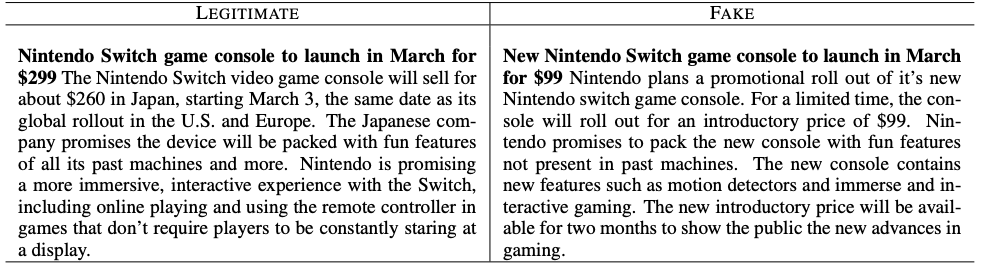
\includegraphics[width=\textwidth]{Results_For_Paper/FakeNewsAMT.png}
  \caption{Example of real and fake news excerpt from FakeNewsAMT}
\end{figure}

The second dataset used in this project was news from the web regarding celebrities. The authors wanted to collect data that naturally arose on the web, rather than using AMT, and believed that collecting news about celebrities granted them an opportunity for fake news, as "public figures ... are frequently targeted by rumors, hoaxes, and fake reports". Legitimate and fake news stories were collected from popular tablod publications, and the legitimacy of a given article was checked using gossip-checking sites and cross-referencing of other articles about the same topic. An example of a real and fake news excerpt is presented in Figure 2.

\begin{figure}[]
  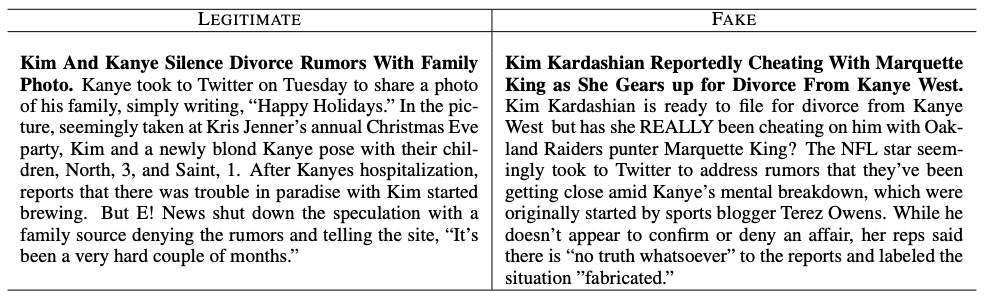
\includegraphics[width=\textwidth]{Results_For_Paper/CelebrityNews.png}
  \caption{Example of real and fake news excerpt from CelebrityNews}
\end{figure}

Moving forward, these two datasets will be called FakeNewsAMT and CelebrityNews, respectively. As a generally summary and in order for the reader to understand the magnitude of the data, see Figure 3, which includes the summary statistics of the two datasets.

\begin{figure}[] 
  \centering
  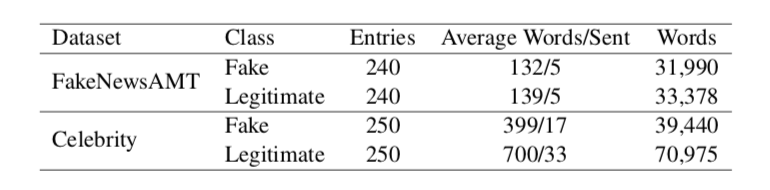
\includegraphics[width=0.7\textwidth]{Results_For_Paper/SummaryStats.png}
  \caption{Summary statistics for the provided datasets}
\end{figure}

The model created in the paper used an SVM and several hand-crafted features. I will go into more detail about the model, the features, and my replication of each aspect in the next section. In general, the features consisted of the words themselves, along with their dependency structures, as well as various natural language based statistics, such as the readability or emotion within the text.

\subsection{Motivation for Replication}

I chose to replicate this project due to both the social importance of the system built by the authors, and the personal intrigue of fake news detection. In terms of importance, I believe the ability to detect misleading information in social media will heavily damper the creation and percolation of fake news itself. With a powerful and accurate metric to detect fake news, there will be little incentive to try and create it in the first place. Unfortuantely, I believe that "fake news" has been repeated so often in mainstream media that it has become somewhat of a joke. Yet, the issue certainly exists in American media. Further, after reading this paper initially and seeing the relative success of the model, I was hopeful that this task of fake news detection may not be out of reach, just one that needs more research investment. Therefore, I wanted to try out making a fake news detection system myself and see the difficulties and possible extensions first hand so that I undestand the process and methods behind similar systems as they start to arise in real-world applications.

On a more personal level, another motivation for this replication task was that I wanted to see the most important features of a model that detects fake news to determine the strength of such a model. That is, I wanted to know how secure this model would be when provided with more intelligently written fake news. In this paper, one flaw is that the fake news creation, while done somewhat thoughtfully, is not necessarily completed with the same motivation as someone writing fake news with a specific purpose and attack in mind. By replicating the project, I could analyze the strengths and weaknesses of the model and determine how it might play out against a stronger opponent, per say. No, this repication project was not all a plot for me to write sneakier, less-detectable fake news - I simply want to know what really seperates the fake from real, and whether the strength of the model is human-interpretable. That is, can this model alert the human reader that the article is fake because there is a lack of punctuation, or will the powerful features be overly abstract and not teach us anything concrete about fake news.

\subsection{Overview of My Task}

My task was to replicate the results completed in this paper. Within his paper, the authors generated two datasets, hand-crafted features for each news article, and ran an SVM on numerous variations of the data. In my replication process, I created the same features as described in the paper and ran all of the same variations of the SVM, but I did not collect new data. The collection of data, as described in the paper, appeared to be a time and resource intensive process. Due to my shortage of time, I decided to use the data collected by the original authors, as it was easily available and allowed me to spend more time on the rest of the replication process. I thought this to be an appropriate exclusion from my project, as data collection, while obviously important, acts more as a difficulty of resources than a technical difficulty. 

\subsection{Layout for this Paper}

With the original paper discussed and my tasks defined, I will now begin discussing the details of my replication process. First, I will discuss the creation of the features, then the creation of each of the results presented in the paper. When discussing the creation of each of these, I will detail the process I took, including all difficulties and failures along the way. In doing so, I will describe the difficulties of the replication process as a whole. After discussing these methods, I will discuss some overall shortcomings and results that I could not replicate. Then, I will discuss potential extensions for this project, although I was not able to complete any myself. Finally, I will finish by outlining the importance of the replicaiton process and my takeaways from this assignment. I will deviate slightly from the outline provided in the official assignment paper, but all of the information will be provided in full. Specifically, the \emph{Feature Creation} and \emph{Model Creation and Results} sections will encapsulate sections 3, 4, and 5 as detailed in the assignment. \emph{Feature Creation} will contain detail on the original work alongside the necessary activities on replication. \emph{Model Creation and Results} will contain detail on the original work, along with the activities of replicating the results, and the replication experiments and results themselves.

\subsection{Quick Note}

It should be noted that throughout my replication process I was able to contact Ver\'onica P\'erez-Rosas, one of the main contributors of this paper. My contact with P\'erez-Rosas allowed me to clarify some ambiguities that existed in the original paper. She did not provided me with any code or anything else that would trivialize the replication process. P\'erez-Rosas was extremetly helpful and I greatly appreciate all of her assistance. 

\section{Feature Creation}

The first coding required task to this project was the creation of all of the features in the paper. The five features used by the authors are Ngrams, Punctuation, Pyscholinguistic features, Readability, and Syntax. I will discuss what each of these features consist of (as detailed in the original paper), and my process for the replication of each feature in this section.

\subsection{Ngrams}

The first feature I needed to create was the Ngrams feature. This feature encodes each provided news article as a tf-idf vector. So, for each article, a vector a \emph{n} unigrams exists, where \emph{n} is the total number of unique unigrams in the corpus. In order to accomplish this task, I used the sklearn preprocessing tools to quickly and easily generate tf-idf vectors for each article, without having to generate unigram counts manually. This tool takes in a corpus and automatically calculates tf-idf vectors. I am unsure if the original authors used this tool as well, but the tool gives quick and accurate results, so I decided to use it.

Upon initially creating the Ngrams feature, my script generated over 20,000 features for both the FakeNewsAMT dataset and the CelebrityNews dataset. In the original paper, the Ngrams feature for the FakeNewsAMT and Celebrity datasets only contained 634 and 1317 features, respectively. I was able to limit the number of features in my feature vector by imposing a threshold on the term frequency. My feature vector now came closer to the number of features presented in the paper. In order to maintain exact replication, I then imposed a max-features limit, so that the tf-idf creation tool only returned a feature vector of the provided length. 

Initially, I did not want to insert a max-features limit, as I thought it was a little close to simply hard-coding a replication. I intended to reach the desired number through combinations of different settings, such as whether to make all letters lowercase, what the term threshold should be, and whether stop words should be counted or not. Through many iterations of setting variation, I could not exactly hit the number of features expected. At this point, I decided imposing the max-features limit is appropriate because it would better allow me to better compare my accuracy to the accuracy presented in the paper. 

My struggles in this section stemmed from a lack of clarity in terms of tf-idf settings in the paper. Initially, I was extremely surprised to be getting a feature vector of greater than 20,000 features, and tried to learn more from the paper but could not. Thresholding the term frequency seemed logical, but it was not defined in the paper.

\subsection{Punctuation}

The next feature to replicate was the punctuation feature. The punctuation feature set consists of "twelve types of punctuation derived from the Linguistic Inquiry and Word Count software (LIWC)". Moving forward, the LIWC dataset will be used numerous times. In order to replicate this feature set, I needed to purchase and download the LIWC software. From there, the LIWC software was very easy to use. The software simply requires the user to enter text files, and then it quickly produces a dataframe that includes every text file, with its filename, and all of the features that LIWC extracts from the text, which is nearly 100 in total. Extracting the punctuation set was as simply as locating the column names for all of the punctuation and simply extracting those columns for each file. The only difficulty in this process was understanding what the LIWC software was and how to use it, but this proved to be quite trivial.

\subsection{Pyscholinguistic Features}

The next feature to replicate was the pyscholinguistic features, which also came from the LIWC software. All of the pyscholinguistic features needed were in the dataframe that was already created for the punctuation feature set. Therefore, the technical aspect of this feature creation was again trivial. Yet, there was some difficulty in discerning the correct LIWC features to choose.

Within the LIWC dataframe output, nearly 100 features exist, and these features do not always have clear subsections. For example, in the paper, the authors broke up the LIWC data into three main categoires: summary categories, linguistic processes, and pyschological processes. In the paper, the authors also provided two examples of what are in these categories. For example, the authors stated that "analytical thinking" and "emotional tone" are part of the summary categories. Yet, in the LIWC dataframe itself, these stratifications do not exist, or at least are not labeled directly. That is, there is no section int he LIWC dataframe labeled summary categories or linguistic processes. There do exist features that match the examples provided (that is, "analytical thinking" and "emotional tone" are present), but to fill out the sections provided in the paper was somewhat of a guessing game.

In order to complete this process, I used the general groupings provided on the LIWC website (http://liwc.wpengine.com/compare-dictionaries/) to make educated guesses. Further, I used the number of features for each feature set, as provided in the paper, as an important piece of information to determine these feature sets. In the end, I am reasonably confident that I created feature sets that were pretty close to the feature sets used in the original paper, but it was impossible to say with a guarantee.

\subsection{Readablity}

The readability feature used a similar solution and also generated a similar problem as the pyscholinguistic features. While not using the LIWC software, the readability features simply existed in an NLP package, and calculating the readability features for each piece of text simply involved inputting text into the readability features package. Yet, a similar problem arised as did in the pyscholinguistic features creation as the readability features function outputted over 40 features, whil only 26 were needed (as provided in the paper). 

I completed a similar process as before, with the LIWC data, to narrow down which features may have been chosen in the paper. Upon my initial guesses, though, the SVM would not fully train on the readability data, due to what I believed to be an issue with the magnitudes of different features. That is, some features existed in the counts of 10,000, while other features were proportions, and thus existed between zero and one. I contacted P\'erez-Rosas, and she claimed this problem did not occur upon her completion of this section. As a result, I deduced that I was selecting the wrong features. So, I iterated through different variations of the the readability features, testing if they were functional, and further, if their accuracies came close to the demonstrated accuracy. I am not as confident that I correctly identified all the correct features, but I do believe I got a solid portion of them. This is one aspect of the project that I wish I had more information on.

One other error I encountered in this process was intial faulty pre-processing of the data. Initially, I pre-processed all of the data, including the removal of stopwords and punctuation. There was nothing said about this in the paper, but I ignorantly thought it was common practice and did it anyway. this caused great error in the readability metrics, as readability is clearly affected by stopwords and punctuation. I do not know what led me to change and eliminate my pre-processing, but it was certainly a error that could have been detrimental to the my results.

\subsection{Syntax}

The final feature, and the most difficulty to replicate, was the Syntax feature. The Syntax feature consisted of "all of the lexicalized production rules" created from context free grammr (CFG) trees. The first difficulty of this task was interpreting the meaning of "lexicalized production rules". The lexacalized production rules of a given word are not clear in the paper, where the authors simply acknowledge that a parse tree is necessary. I contacted P\'erez-Rosas for more information, and she provided me a paper (http://www.aclweb.org/anthology/P12-2034) to learn more about this process. Still confused, I had to further clarify with P\'erez-Rosas to ensure that I was extracting the correct information. Upon ultimate clarification, I came to the conclusion that the information necessary for extraction was various combinations of a word, its CFG parent and its CFG grandparent.

Next, in order to gather the information required for this feature set, it was necessary to run the Stanford Parser on every article in the dataset. The Stanford Parser, to my knowledge, does not directly provide the information necessary for this feature set. Thus, I had to creatively parse the output to get the correct lexicalized rules. This took several attempts, but my final result seems to accurately extract the production rules. Upon deep investigation of my results, I find some pieces of information that I know to be incorrect, but, due to their low frequency, they will be filtered out upon the creation of tf-idf vectors for this information. 

Due to the nature of this problem, I was unable to use the same sklearn tf-idf vectorizer, but rather had to save counts of different terms in order to manually calculate the tf-idf values of each term in each sentence. Further, there were some pieces of text that were unable to generate parse trees when pased into the Stanford Parser. As a result, I had to fill in the missing values for these articles. For both the FakeNewsAMT and the CelebrityNews datasets, the proportion of invalid articles fell below 5 percent. As a result, I found it appropriate to simply fill in the tf-idf values of the invalid articles with the averages of tf-idf values from every other instance. Since the number of invalid articles was so low, I do not expect this to have a significant impact on my results.

For this feature set, I was unable to exactly replicate the number of features presented in the original paper's version of the CFG feature set. My feature sets consist of 1250 and 3242 features for FakeNewsAMT and CelebrityNews, respectively, while the original paper has feature sets consisting of 1377 and 2599. I plan to continually work on this, but also do not expect it to be a great impact on my results.

All in all, this feature set proved to be the most difficult for several reasons. First, the description in the paper of the actual information needed is relatively vague, and had I not contacted the author I would have been extremely lost. Second, the use of the Stanford Parser provides complications due to the complexity of that software, and the ambiguity of its use with respect to this project. Finally, the lack of tf-idf settings again leads me to sizes of feature sets that do not identically match the sizes of the feature sets presented in the paper.

\subsection{Feature Creation Summary}

Due to certain ambiguous descriptions of features within the paper, the feature creation process caused various issues and I conclude with certain feature sets that I am not fully confident of their fidelity to the original paper. For the most part, I believe most feature sets have the bulk of the necessary information, if not all of it, and will perform well when run in the model. Yet, this process of feature replication made me further understand the difficulty of replication as a whole, as there are many small details that go in to creating features and training models that may not be relevant for a paper but are extremely relevant when attempting to conduct the same experiment.

\section{Model Creation and Results}

With all the features created, I moved on to running the variations of models presented in the paper. The model used throughout this paper is a linear SVM classifier using the default features in the caret and e1071 packages. These packages exist in R. I had been completing the replication process in Python, not R, and wanted to continue my process in Python. I researched both the R packages used in the original study, and then researched the scikit-learn SVM function - a commonly used implementation of SVMs in Python - and found they were quite similar in implementations. The R package uses LibLinear, while the scikit-learn version uses LibSVM. Upon research of the differences in these packages, I found moderate changes in certain parameters, but nothing significant enough to demand I use LibLinear to ensure correct results. Therefore, I continued using Python and scikit-learn based on educated research of the comparisons between the two technologies. 

In the rest of this section, I will walk through each of the Tables and Figures presented in the paper. I will detail the process of replicating these Tables and Figures, including the challenges and failures, and finally present the results I obtained alongisde the real results.

\subsection{Replication of FakeNewsAMT Classification}

The first results presented in the paper are in Table 4, captioned "Classification results for the FakeNewsAMT dataset". The results in this table display the accuracy and F1-scores of training and testing the model on each feature set independently, and then all of the feature sets together. As specified in the caption, this table is trained and tested on the FakeNewsAMT dataset. This table was relatively straightforward, as it simply involved using the feature sets I had just created and training a very simple SVM on the data. Upon running the model initially, I was obtaining slightly different results each time I ran the model. With this in mind, I decided to add multiple runs and take averages. Time was not an issue in the process of generating this table, so I was able to get many runs for low cost. In the original paper, there is no mention of various runs, and thus I have less of an idea of the variance involved in the results presented. This issue of a lack of presented variance exists throughout the paper, and I will talk about it more later. The results for my replication and for the original paper are presented in Figures 4 and 5.

\begin{figure}[]
  \centering
  \begin{minipage}[b]{0.4\textwidth}
    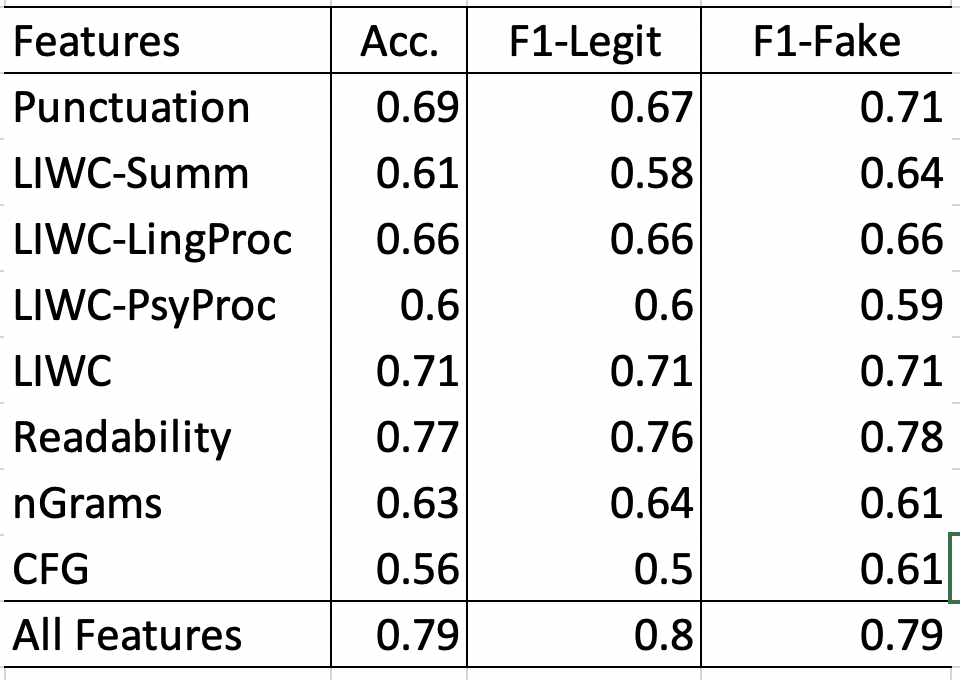
\includegraphics[height=4cm, width=\textwidth]{Results_For_Paper/Table4Me.png}
    \caption{My Replication's classification results for the FakeNewsAMT dataset}
  \end{minipage}
  \hfill
  \begin{minipage}[b]{0.4\textwidth}
    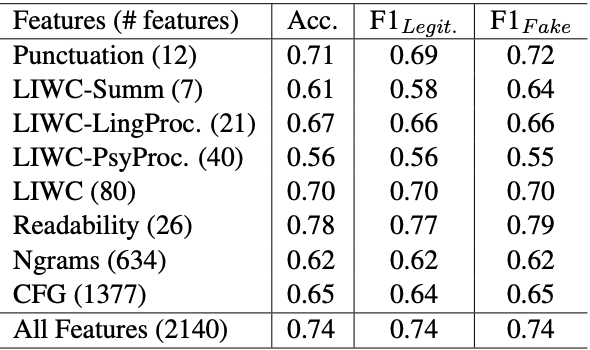
\includegraphics[height=4cm, width=\textwidth]{Results_For_Paper/Table4Real.png}
    \caption{Original Paper's classification results for the FakeNewsAMT dataset}
  \end{minipage}
\end{figure}

For Table 4, nearly every value is roughly the same as the original value other than the values calculated for CFG and the values calculated for All Features. For the CFG feature, the error comes from the creation of the feature data set, as described in the above sections. This feature was difficult to create due to use of complex technologies and ambiguity in the original paper about what this feature consisted of. Without any ground truth of the feature set to compare my feature set too, I am unsure if the feature set I created identically matches the one used in the original paper. I have contacted P\'erez-Rosas to help gain information, so hopefully I will be able to correct this in future iterations of my replication. As for the All Features feature set, I am scoring higher than the original paper by a seemingly significant margin. While I am unsure as to why this difference exists, I also have no motivation to change it, as my model performed better than the original model. I made sure that I was not somehow getting a better accuracy by cheating in some way, like providing my model with more information than was provided to the original paper, but found nothing out of the ordinary. 

\subsection{Replication of CelebrityNews Classification}

The replication of Table 5 involved in the exact same process as Table 4, but using the CelebrityNews dataset rather than the FakeNewsAMT dataset. The results for my replication are displayed in Figures 6 and 7.

\begin{figure}[]
  \centering
  \begin{minipage}[b]{0.4\textwidth}
    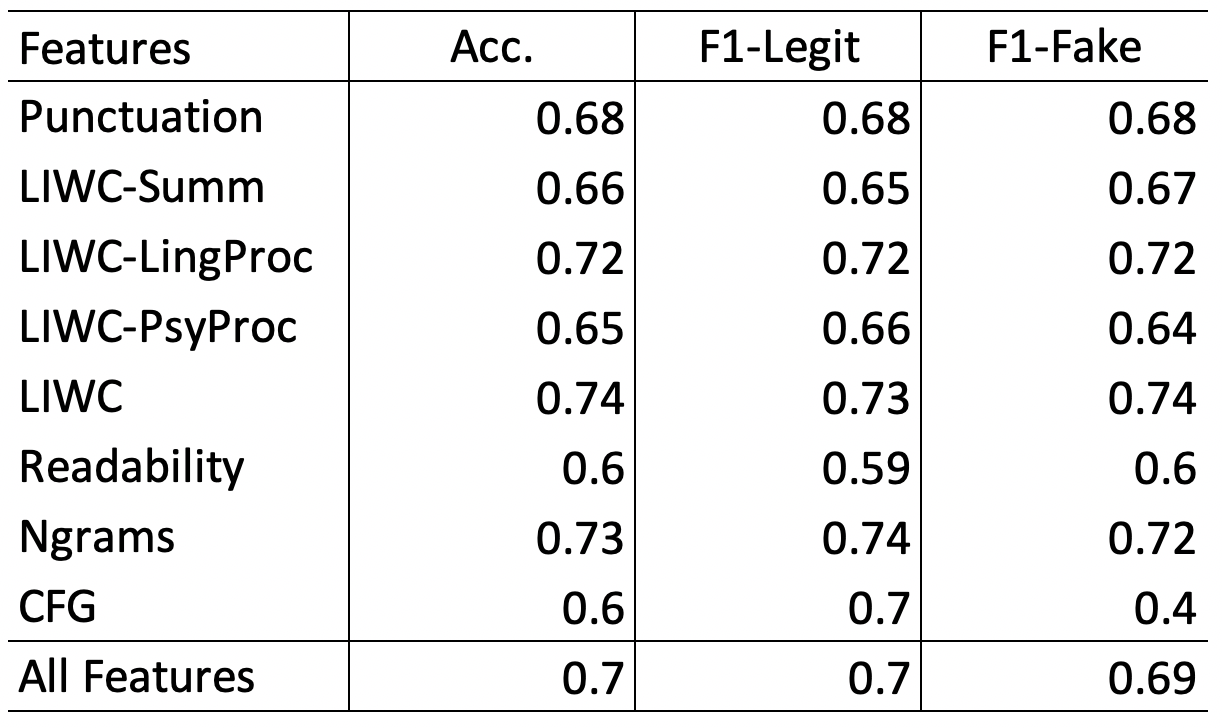
\includegraphics[height=4cm, width=\textwidth]{Results_For_Paper/Table5Me.png}
    \caption{My Replication's classification results for the CelebrityNews dataset}
  \end{minipage}
  \hfill
  \begin{minipage}[b]{0.4\textwidth}
    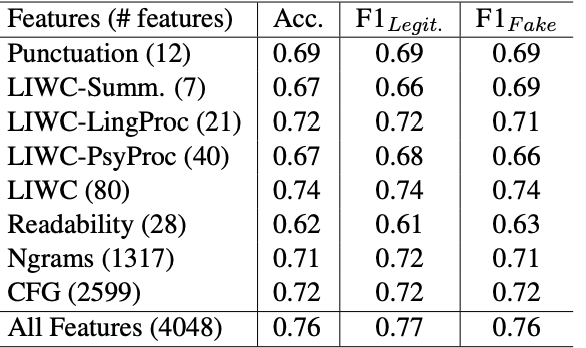
\includegraphics[height=4cm, width=\textwidth]{Results_For_Paper/Table5Real.png}
    \caption{Original Paper's classification results for the CelebrityNews dataset}
  \end{minipage}
\end{figure}

Again, the feature sets that are incorrect in my replication are the CFG feature set and the All Features feature set. The CFG feature set displays an egregiously different F1-Fake value, while the accuracy and F1-legit values are a little less variant. I continue to connect this difference to the creation of the feature set, and will hopefully better this moving forward. As for the All Features set, I am unsure at the difference in results. Since all other categories look mostly similar, I should think that the All Features category should also match up relatively well. I worry that the impact of the deprecated CFG feature set is great enough to negatively affect the All Features set. Even so, the values are within 10 percent of each other and may be a product of variance. I do not think this is certainly the case, but I figure the issue lies somewhere in between variance and incorrectly created feature sets. Notably, when I try running my model using only 1 run, and thus not averaging multiple runs through the model and the dataset, I have seen, at the maximum, the All Feature set return an Accuracy of 0.73, an F1-legit of 0.73, and a F1-fake of 0.73. These values still do not directly match the values presented, but do demonstrate the existing variance and the possibility that the authors used their best result as their published result.


\subsection{Replication of Incremental Training Data Usage Learning Curve, FakeNewsAMT}

Figure 1a in the original paper presents the evolution of the accuracy of the model when using more data for training. That is, the model if first trained on 20 percent of the data, then 40, increasing by 20 all the way to 100 percent of the data. The importance of these figures is in showing the value of more data with respect to this study. For the most part, the replication of these figures were relatively straightword, as it involved running the same model as needed for tables 4 and 5, just simply using less of the data. One decision I made that was not indicated in the paper was the decision to take stratified samples of the data, when necessary. The dataset as a whole consisted of equal amounts of legitimate and fake data. When taking 20 percent of the data, for example, I thought that taking a sample that maintained this 50/50 split of data would help reduce variance in the results. The variance would reduce in this case because there would not be one run that only trained and tested on legitimate data, while another was only trained and tested on fake data. A situation like this may create extremely different models and different summary statistics. So, while this method was not mentioned specifically in the paper, I found it to be a valid method to implement in my replication. Using the stratified split, and otherwise using the same linear SVM as used before, I obtained the results displayed in Figure 8, and the results from the original paper are displayed in Figure 9.


\begin{figure}[]
  \centering
  \begin{minipage}[b]{0.4\textwidth}
    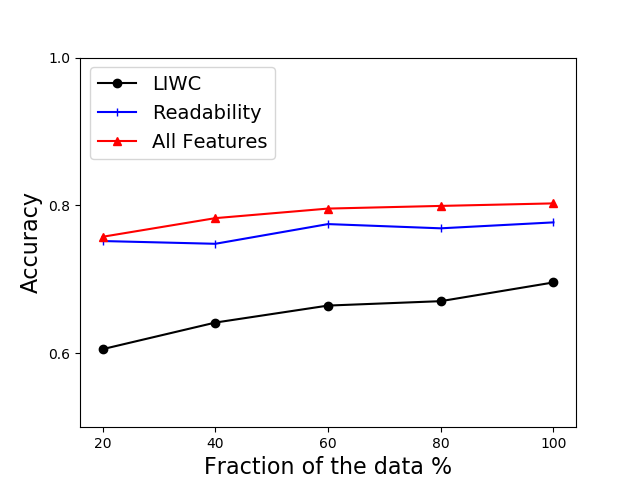
\includegraphics[width=\textwidth]{Results_For_Paper/Figure1a-me.png}
    \caption{My Replication's learning curve using incremental fraction of the data and three feature sets for FakeNewsAMT dataset.}
  \end{minipage}
  \hfill
  \begin{minipage}[b]{0.4\textwidth}
    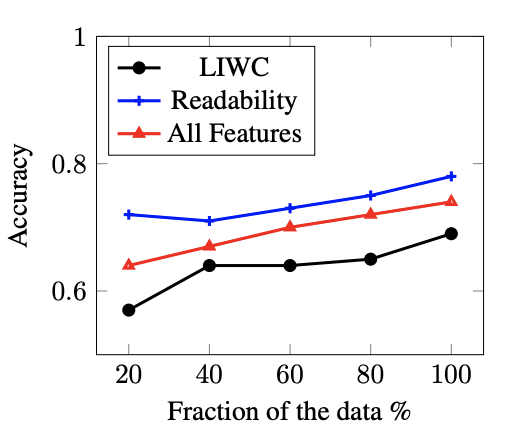
\includegraphics[width=\textwidth]{Results_For_Paper/Figure1a-real.png}
    \caption{Original Paper's learning curve using incremental fraction of the data and three feature sets for FakeNewsAMT dataset.}
  \end{minipage}
\end{figure}

Starting with the LIWC feature set, the replication pretty closely mirrors the result presented in the original paper. When only 20 percent of the data is used, my replication scores  higher than what is presented in the paper. Yet, for the rest of the points, both graphs exhibit an upward trend from 40 percent to 100 percent, and both end up around a 65-70 percent accuracy. The All Features feature set exhibits the same shape in both graphs, but the accuracy is higher in my replication. This difference was already discussed in the section detailing the replication of Table 4. While the numbers are off, the trend is monotonically increasing in both graphs, even if insignificantly. Finally, the Readability feature set exhibits very similar values at each X-value, and the general trend of increasing accuracy exists in both graphs. In my replication, a spike exists at the 60 percent X-value, but other than that we see accuracy increase. With the small amount of difference in accuracy in every point, it is also expected that the variance that exists in these results may push these points around. In general, and as mentioned before, error bars in the original paper would have helped clarify these values a little more. Either way, both my graph and the original graph display general upward trends as more of the data is used, which was the important point taken away from this aspect of the paper.

\subsection{Replication of Incremental Training Data Usage Learning Curve, CelebrityNews}

The replicaiton strategy was the exact same for Figure 1b as it was for Figure 1a. The results for this replication process are displayed in Figures 10 and 11.

\begin{figure}[]
  \centering
  \begin{minipage}[b]{0.4\textwidth}
    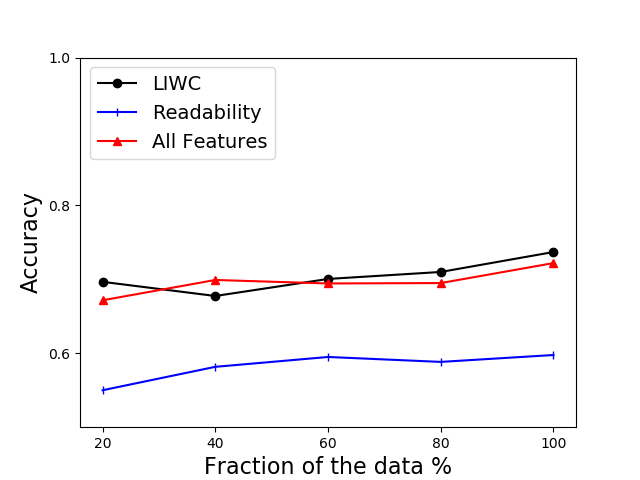
\includegraphics[width=\textwidth]{Results_For_Paper/Figure1b-me.png}
    \caption{My Replication's learning curve using incremental fraction of the data and three feature sets for CelebrityNews dataset.}
  \end{minipage}
  \hfill
  \begin{minipage}[b]{0.4\textwidth}
    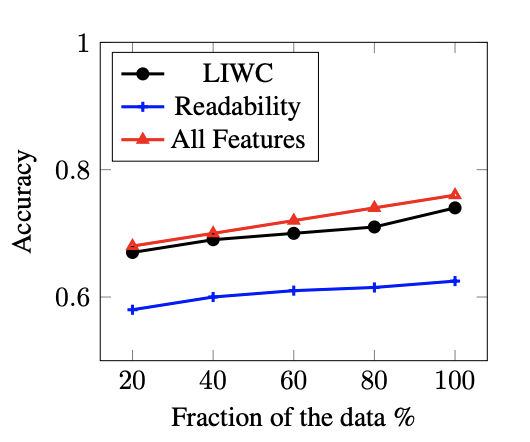
\includegraphics[width=\textwidth]{Results_For_Paper/Figure1b-real.png}
    \caption{Original Paper's learning curve using incremental fraction of the data and three feature sets for CelebrityNews dataset.}
  \end{minipage}
\end{figure}

Starting again with the LIWC feature set, my replication graph exhibits a very similar trend as the original paper, and, with some variation, is nearly identical. The same applies for the All Features feature set, as the values and trend are nearly identical, with the main difference being the values themselves. We see the values in my replication are less than the values in the original paper, but this was already discussed in the creation of Table 5 subsection. The general trend of an increasing accuracy exists in both graphs, though, for the All Feature feature set. Finally, the Readability feature set is more stagnant in my replication data than in the original data. My data does not exhibit much of an increase when more data is added to the model, but rather stays nearly the same as the accuracy when using 20 percent of the data. I have no intuition as to why this may be the case, but, at the same time, the increase from 20 to 100 percent of the data in the original graph is not much different itself. All in all, this graph displays similar trends and data points as the graph created in the original paper, with some modifications. 

\subsection{Replication of Cross-Dataset Analysis}

Table 6 in the original paper consisted of training the SVM on one dataset (FakeNewsAMT or CelebrityNews) and testing on the other dataset. The idea was to determine if the two types of news shared similar defining features for the detection of misleading information. In order to properly train the models, it was necessary to first create new Ngrams and Syntax feature sets that contained all the words from both datasets. By making new feature sets, the input for each of these feature sets from both datasets will be of the same size, which is necessary for an SVM. Another way of ensuring that the input for these feature sets are the same size for testing and training is to map the testing set to the features of the training set. That is, use the features of the training (unique words, for an example using Ngrams), and simply make a tf-idf vector for the testing data based on these unique words. The problem here is that it is possible that many words that exist in the testing data do not exist in the training data, and vice verca, and may not properly encapsulate all the data. This issue, along with the simplicity of the first method presented, lead me to complete this task using the first method of creating a combined Ngrams and Syntax feature sets. Using this method, and then training a simple linear model on the training data (as before) and testing on the other dataset, I produced the results displayed in Figure 12, and the results produced by the original authors are displayed in Figure 13.

\begin{figure}[b]
  \centering
  \begin{minipage}[b]{0.4\textwidth}
    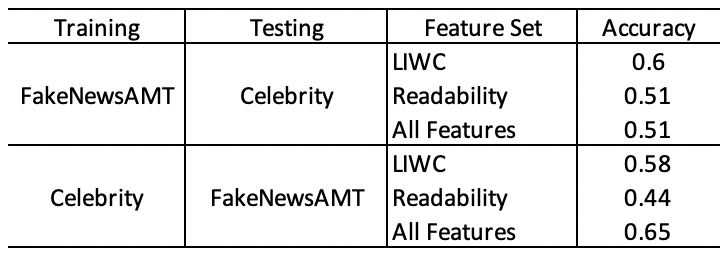
\includegraphics[width=\textwidth]{Results_For_Paper/Table6Me.png}
    \caption{My Replication's cross-domain analysis for best performing feature sets.}
  \end{minipage}
  \hfill
  \begin{minipage}[b]{0.4\textwidth}
    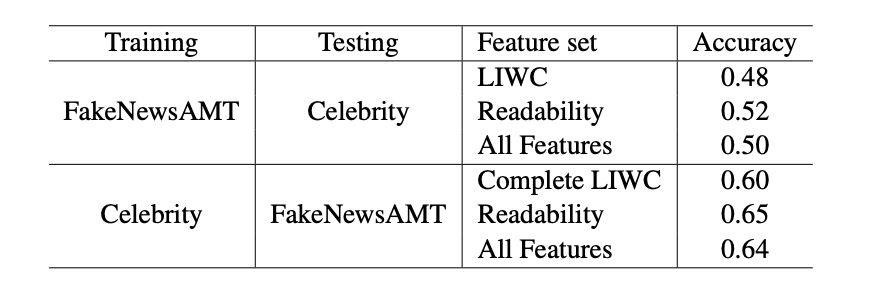
\includegraphics[width=\textwidth]{Results_For_Paper/Table6Real.png}
    \caption{Original Paper's cross-domain analysis for best performing feature sets.}
  \end{minipage}
\end{figure}

When comparing the results, we observe differences when training on FakeNewsAMT with the LIWC feature set, and when training on Celebrity with the Readability feature set. For the first difference, my model produces an accuracy of 0.6, compared to the accuracy of 0.48 in the original paper. For the second difference, my model produces an accuracy of 0.44, compared to the accuracy of 0.65 for the original paper. All other accuracies match (or are at least close enough). I am unsure as to what caused the differences between my results and the results presented. 

\subsection{Replication of Cross-Domain Classification}

Table 7 in the paper breaks down the FakeNewsAMT dataset into six domains - Technology, Education, Business, Sports, Politics and Entertainment - in order to test if the different domains display different accuracies. The authors chose only to test certain features for each domain, in this case they tested Readability, LIWC and All Features. The method of testing the different domains was to exclude a given domain from training, so use the other 5 domains to train the model, and then test on the single domain. This process was not too difficult to replicate, as it simply involved seperating the data and performing simple training and testing processes. The table of my replication and the table from the original paper are presented in Figures 14 and 15, respectively.

\begin{figure}[]
  \centering
  \begin{minipage}[b]{0.4\textwidth}
    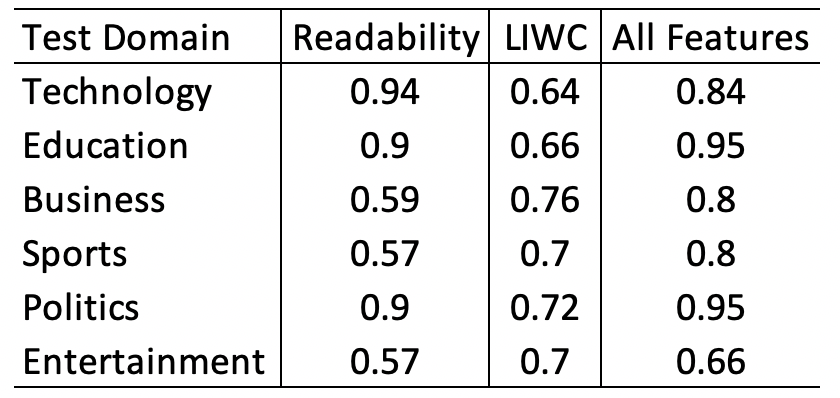
\includegraphics[width=\textwidth, height=3.5cm]{Results_For_Paper/Table7Me.png}
    \caption{My Replication's cross-domain classification accuracy for certain feature sets. Using FakeNewsAMT dataset.}
  \end{minipage}
  \hfill
  \begin{minipage}[b]{0.4\textwidth}
    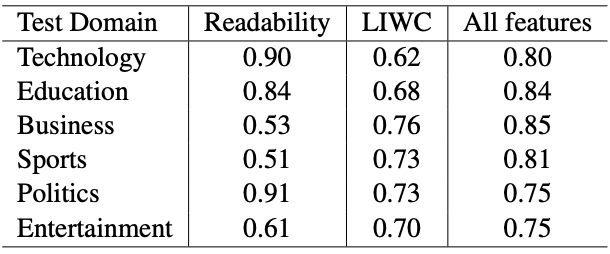
\includegraphics[width=\textwidth, height=3.5cm]{Results_For_Paper/Table7Real.png}
    \caption{Original Paper's cross-domain classification accuracy for certain feature sets. Using FakeNewsAMT dataset.}
  \end{minipage}
\end{figure}

Many of the values I got for my replication were relatively similar to the values produced in the original paper. Specifically, the domains of Technology, Business, and Sports all produce roughly similar results, if not a little better. For the Education and Politics domain, my replication process produces significantly better results when testing on All Features. Similar to my explanation when describing my better results for Table 4, I did not feel the need to change my process in order to attempt to create worse results. I thoroughly investigated my process of training and testing the models, and did not find that I "cheated" anywhere, in the statistical sense, and thus did not find a way to try to perfectly replicate these inferior results. Specifically for the Politics domain, the All Features accuracy result obtained in the original paper of 0.75 confused me, as the Readability domain itself produced an accuracy of 0.91. The model that includes All Features, including the Readability feature, should seemingly not score that much lower than the Readability feature on its own. Finally, the accuracies from my model for the Entertainment domain differed from the corresponding domain in the original paper, specifically the All Features domain (0.66 accuracy in replication, 0.75 accuracy in replication). I struggled to determine the cause of these differences in accuracy. My main struggle was finding a way to potentially alter the accuracies that were incorrect, while maintaining the majority of accuracies that were correct. By changing the model slightly, I would alter all the accuracies, and with most of them already being correct (correct with respect to replication, that is), I decided to not change my model and accept that I have a different answer for an unknown reason. I will discuss this decision, and others like it, more in later sections. 

\subsection{Unreplicated Tasks}

Now that I have discussed and presented all of my replication tasks, I think it is important to quickly note the parts of the original paper that I did not replicate. I chose not to replicate the creation of the dataset (as discussed earlier), Table 8, and Table 9. Tables 8 and 9 display comparisons between the created system and human annotators. The importance of this section is to display the ability of the system with directr comparison to human annotators who are attempting to discern news as fake or real. Involved in creating these tables was getting a group of real humans to spend a large amount of time classifying news as real or fake. Due to a lack of resources and time, I could not get a group of human annotators to classify each news article. Further, this aspect of the paper requires minimal technical ability, and thus is not necessary for replication. Given that the annotated data already exists and is present in their paper, I could simply use their data as a baseline myself.

\section{Extensions}

Due to the large amount of work involved in this replication process, including the replication of all features - which took significantly longer than expected due to ambigious feature descriptions and new technologies - and the large amount of experiments (6 total), I was unable to complete any extension myself. However, I am do have several ideas for extensions that I would have attempted had I finished earlier, and may still complete after the end of this class.

The first extension I propose is the identification and interpretation of the results with respect to the most informative features. I discussed this briefly in the introduction as well, but I think an important result for the detection of fake news using automated systems is not only the classification of real or fake, but the \emph{description} of real or fake. In other words, \emph{why} was a certain enws article classified as fake. Using the information of \emph{why}, humans will be better at the identification of fake news themselves, perhaps. There is a possibility that the features that help identify fake news will be overly abstract to the human mind. For example, we see that the Readability feature set performs well, but expecting a human to be able to identify Readability metrics may cause issues.

Another extension would be to carry over the given model to the comparison of different sets of text. For example, I could imagine using this model, possibly with some modifications, to compare and contrast the writing styles of different figures. For example, I could run a similar model to determine how my writing differs from the writing of certain authors, and determine the main stylistic choices that differ. If the model can determine the difference between the two writing, it can hopefully translate the main differences into a useful way. This is especially true when using a linear kernel for SVM's, as other kernels such as RBFs would not allow for easy interpretation.

In general, I ideally would extend this project to make it more than just a blackbox tool for classification, but rather an informative tool on how to identify fake news, or how to identify specific writing styles in general. I think a lot of information is embedded in the models created throughout this paper, and there lies a lot of importance in extracting and interpreting that information.


\section{Discussion on Differences}

Throughout this paper, I have displayed numerous differences between the results I produced and the results displayed in the original paper. Many of these results that slightly differed may be, and most likely are, just an issue of variance. Due to the lack of variance bars or any description in general within the original paper, it is impossible to say for sure that may results are within a reasonable amount of the results in the paper, but I can confidently say that they are. So, then, it is reasonable to say that I successfully replicated many of the results produced in the paper. 

Even so, there were a few accuracy results where my replication process produced a significantly different result. Namely, the results for the CFG feature in both Figures 4 and 5, and 6 and 7,
the trend of the Readability feature presented in Figures 10 and 11, the previously pointed out differences in Figures 12 and 13, and the Entertainment with All Features accuracy presented in Figures 14 and 15. I will quickly go through each of these differences, although I may have discussed some previously in the paper.

For the CFG feature sets in Figures 4, 5, 6, and 7, I discussed the potential cause of this issue stemming from the confusion as to what this feature set should really consist. The "lexacalized production rules", as discussed in the paper, are not extremely clear, and even after my correspondence with the authors I still find this feature difficult to understand. I plan on continuing to follow up with the authors about this feature set, as it is the only feature set I am not confident about its successful recreation.

For the Readability features in Figures 10 and 11, the mismatching features in Figures 12 and 13, as well as the Entertainment accuracies in Figures 14 and 15, I find myself questioning the authors a little more than I did on the other differences between my results and the results of the paper. In both of these instances, the rest of the results in the respective replications of these Tables / Figures appear correct. That is to say, my method of implementation is clearly not entirely faulty, as my method produces the correct results for nearly every other instance of the problem. Therefore, I find it difficult to imagine that my replication process somehow went awry for these seemingly random instances. I find it reasonable that I may have small errors that compounded in these specific errors, but I also feel confident in my answers. My response here is to say that I am genuinely interested to know how we got such different answers, given that most of our other answers were so similar. This is what has interested about this project, is the cases where the results differ but for reasons that are extremely difficult to determine. As stated earlier, I chose not to extensively try to manipulate my models in order to change my results, because then I would just be cheating to match a result, rather than implementing a system based on what I think the real system looks like. I think it is okay that our results differ slightly, and I would hope that someday I get to learn why, if that is possible. I will elaborate further on my takeaways from this project in the next section.

\section{Conclusions and Lessons Learned}

Going in to this project, I did not entirely know what to expect. As someone who has never attempted any sort of replication, I thought it could go one of two ways. First, it would be extremely simple, because the paper could be detailed and well documented, enough for me easily recreate the features and models at hand. But, on the contrary, I thought it may prove to be very difficult if I do not get the same results and no further resources exist to question my replication. That is, in all classes throughout my computer science educational career, there was one right answer, and there were people who knew exactly how to get to that answer (professors, GSI's, other classmates). In this replication project, there were few resources beyond the text itself to help me hurdle my issues.

Interestingly for me, my replication attempt took on both the simple and the difficult form. In its simple form, I was able to run certain models with some of the easier to create features and immediately get a nearly perfectly replicated result. For certain figures and tables, I generated them one time and never needed to modify anything. Yet, for certain other aspects, I obtained different results, and, connected to the difficult part of the project, had nowhere to turn. Luckily, I had one of the author to contact for basic questions, but these interactions were rather limited and the answers provided were non-exhaustive (and I mean no disrespect to the authors, because any answer was more than is expected from them and provided me great help regardless). So, without many resources to turn to, I was left to strictly analyze my methods and cycle through all my past projects and coding experiences to determine what I could add, subtract, or modify from my system to more closely match the system at hand. 

For some portions of the project, such as adding a threshold for tf-idf calculations or sampling from a stratified sample for incremental training data, I was able to use my past knowledge productively and solve the problem. Yet, many parts, as discussed, remained different from the published results. And now, this difference in results presents a new problem that only exists in replication. In homework assignments and school projects, a correct answer does exist, and you have to find a way to find that answer. When replicating another project, the results the original authors produce is not necessarily correct. In many ways, this is the reason for replication in the first place. Yet, it also constantly poses a question to the replicating author (me): my answer is not the same as the original answer, so should I continue to alter my system to match the original or should I accept my result as different? The answer to this question obviously varies by case, but it presents a dilemma that I had not yet faced in my scholastic career.

All in all, I greatly enjoyed this project because it presented a new type of problem that I have no experience with. I have experience with scholastic projects, where one right answer exists. I have experience with professional projects, where no right answer necessarily exists. But replication offers a strange middle ground, where an idea of an answer exists, and you certainly strive to recreate the existing answers, but if some answers do not exactly match, it does not necessarily deem your answer incorrect. It further taught me how to more deeply analyze a paper, and what details of a paper are more necessary than others.

\section{Final Notes and Acknowledgement}

Professor Laird, I have greatly enjoyed this class and feel that I have learned a lot. I now feel more comfortable  reading research papers critically, presenting research papers in detail, and participating in discussions regarding a wide range of AI topics. I want to thank you for a enjoyable semester in this class. I think you made the class fun and not intense to a point where students felt relaxed enough to present and speak, but also intellectual and legitimate, so that the conversations and presentations had an expectation of sophistication. This class, and this year in total (I was in 592 in the fall) has truly satisfied my desire to learn about Artificial Intelligence, and I thank you greatly for that.


\end{document}










